\documentclass[10pt,letterpaper]{article}
\usepackage{graphicx}
\usepackage[utf8]{inputenc}
\usepackage[spanish]{babel} 
\usepackage{amsmath}
\usepackage{amsfonts}
\usepackage{amssymb}




\begin{document}
\begin{titlepage}
\begin{minipage}{12cm} Universidad de Chile
\\ Facultad de Ciencias F\'isicas y Matem\'aticas
\\ Departamento de Ciencias de la Computaci\'on\\
\\
\end{minipage}
\vspace*{2cm}
\begin{center}
\vspace{0.2cm}
{\Huge\bf\vspace{0.5cm} Informe de Trabajo Dirigido}\\
{\Huge\bf\vspace{0.5cm} Desarrollo de una Aplicación con Georreferenciación para Android}\\
\end{center}
\vspace{4cm}
\begin{tabular}{ll}
\bf{Nombre Alumno :}& Jorge Romo J. \\
\bf{Carrera:} & Ingeniería Civil en Computación\\ 
\bf{Profesor:} & Jeremy Barbay  \\ 
\bf{Correo Electrónico:} & jromo.dcc@gmail.com  \\ 
\bf{Fecha:} & 22 de Junio de 2011  \\ 
\end{tabular}
\end{titlepage}
\newpage
\tableofcontents
\setcounter{tocdepth}{1}

\newpage
\section{Introducción}

El presente informe consiste en una descripción del trabajo realizado para desarrollar y estudiar la usabilidad de una aplicación para el sistema operativo Android, que utilice georreferenciación como base de la misma.\\

Este proyecto tuvo su inicio como una idea para participar en el Concurso Universitario de Aplicaciones para Android realizado por Cursor Labs, posteriormente, viendo los buenos resultados que obtuvo el proyecto en el concurso (2do lugar), y el interés sucitado por el mismo entre los otros participantes, profesores, y además entre alumnos de la Escuela de Verano de la Universidad de Chile, a quienes se les realizó una presentación acerca de la aplicación, se estimó que el proyecto tiene bases para continuar, y para ello, se reformularon los objetivos y la propuesta como tal.\\

Se decidió comenzar realizando una encuesta a distintos usuarios que estuviesen dentro del público objetivo de la aplicación, para luego, a partir de los resultados obtenidos, elaborar un prototipo que permitiese realizar un estudio de usabilidad del mismo, para reformular los objetivos y el enfoque de la aplicación de acuerdo las conclusiones obtenidas, a partir de las opiniones recibidas por los usuarios.\\

A continuación se presentan, en primer lugar, el objetivo general de la aplicación, una descripción de las aplicaciones de este tipo ya existentes, los resultados de la encuesta previa realizada a los usuarios, para luego describir detalladamente la propuesta de prototipo de la aplicación, los resultados del estudio de usabilidad del mismo, y los avances en un segundo prototipo basado en dichos resultados. Además, se describe a grandes rasgos lo que se pretende realizar a futuro en este proyecto, fuera del alcance de este trabajo dirigido.\\

\newpage
\section{Descripción del Problema y Objetivo General de la Aplicación}

Existen muchas aplicaciones que utilizan la georeferenciación en los smartphones y/o tablets, no obstante, ninguna de ellas logra dar información que los usuarios consideren confiable, o bien, si lo hacen, se debe sacrificar la interación de los usuarios con la misma o sus posibilidades de aportar información a la misma aplicación, o incluso se pierde el objetivo para el cual fueron concebidas, es decir, los usuarios las utilizan de una forma que claramente no era la deseable.\\

Lo que se busca mediante la aplicación a desarrollar, es tener un buen balance entre permitir a los usuarios aportar información para mejorar la aplicación, que obtengan beneficios dentro de la misma a medida que colaboren, pero garantizando que la información aportada sea confiable.\\

Para ello, la propuesta es que los mismos usuarios realicen la validación del contenido al utilizar la aplicación, mediante la resolución de desafíos que consistan en preguntas que permitan validar si la información aportada por otros usuarios es correcta.\\

A continuación se describen aplicaciones con georreferenciación frecuentemente usadas (como se ve en la encuesta previa, más adelante), resumiendo sus ventajas y desventajas, para reflejar lo descrito anteriormente:\\

\subsection{Aplicaciones con Georreferenciación}

\begin{itemize}
 
\item \textbf{Foursquare}\\

La aplicación tiene el objetivo de dar a conocer lugares, y que los usuarios los evalúen dándoles puntaje, utilizando la georreferencia para comprobar que los usuarios efectivamente estuviesen ahí. Para motivar a los usuarios a usar la aplicación, ésta otorga medallas o categorías de “alcalde” de un lugar, lo cual se puede compartir a través de las distintas redes sociales. No obstante, esto lleva a que finalmente se pierda el objetivo inicial de la aplicación, ya que en general los usuarios intentan ir muchas veces a un mismo lugar para ser alcades, o crean lugares nuevos para ganar medallas, por lo cuál muchas veces no se utiliza de la manera esperada.\\

\textbf{Features:}\\
\begin{itemize}
\item Puntaje y comentarios de los lugares
\item Agregar nuevos lugares
\item Marcar lugares como visitados
\item Obtención de medallas por visitar lugares
\item Se puede compartir los lugares visitados por las redes sociales
\end{itemize}

\textbf{Limitaciones:} No existe ningún tipo de validación de los lugares agregados, puedo visitar varias veces el mismo lugar (incluso mi propia casa), para intentar obtener medallas.

\item \textbf{Google Maps}\\

Además de servir como un mapa, muestra lugares destacados como restaurants, sitios históricos, etc. y también servicios tales como el Metro. No obstante, se utiliza más para ubicarse, encontrar calles, saber donde se está, etc. que para dar a conocer nuevos sitios, o saber que lugares visitar.\\

\textbf{Features:}
\begin{itemize}
\item Datos de casi todos los servicios de las ciudades, clasificación muy minuciosa de los mismos.
\item Distintas vistas de la ciudad (satelital, calles, etc.)
\item Permite realizar búsquedas por dirección en el mapa
\item Se pueden agregar fotos de lugares
\item Se puede realizar "check-in" o rankear lugares visitados
\end{itemize}

\textbf{Limitaciones:} Existen alternativas Open Source locales más precisas (Ej: Open Street Map, grupo en Chile: http://www.openstreetmap.cl/). No existe validación para las fotos que se agregan, no hay premios ni incentivos para que el usuario realice aportes. En general, es una aplicación más orientada a "ver" el mapa para ubicarse, que a buscar interacción de algún tipo con el usuario, por lo mismo, la información de ubicación de lugares que tiene, es altamente confiable, por lo que es muy usada.\\

\item \textbf{Ovi Maps}

\textbf{Features:}
\begin{itemize}
\item Mapas Descargables, ya sea por WiFi al usarlo en el equipo móvil, o bien descargándolos en un pc de escritorio y subiéndolos al celular, ambas alternativas permiten que pueda funcionar en Modo Offline.
\item Búsqueda de direcciones
\item Utilización de GPS como sistema de navegación
\item Compartir localizaciones mediante redes sociales
\item Opción de programar alertas vibrantes
\end{itemize}

\textbf{Limitaciones:} No existe forma de que los usuarios aporten nuevos lugares, o de evaluación y recomendaciones de los mismos.\\

\item \textbf{RunKeeper}\\

Aplicación orientada a deportistas, en particular corredores, que permite guardar las rutas realizadas. Éstas se pueden compartir y comparar con otros usuarios de la aplicación, de tal forma que se puede, por ejemplo, realizar desafíos de tiempo para una ruta en particular.\\

\item \textbf{SCVNGR}\\

Aplicación que permite a los usuarios resolver desafíos ubicados en distintos lugares (Locales de comida, universidades, plazas, etc.), los cuales son proporcionados por la empresa que ocupa el lugar, y a cambio de resolverlos se obtienen medallas o premios reales como descuentos en el local.\\
\textbf{Ejemplo:} McDonalds pone un desafío en uno de sus locales. La interfaz de la aplicación indica que hay un desafío en el local, y al hacer click aparece un origami, si vas al local y sacas una foto con tu móvil de la servilleta con el origami hecho, tienes una bebida gratis.\\
\textbf{Limitaciones:} Los lugares disponibles, y por supuesto, los desafíos, son impuestos por las empresas, los usuarios no pueden agregar nuevos lugares o desafíos.
\end{itemize}

\newpage
\section{Objetivos del Trabajo Dirigido}

El Objetivo del presente trabajo es realizar un estudio acerca de la aplicación de geolocalización Tripdroid, para determinar el enfoque que se le debe dar y las características que debe tener. Esto mediante la opinión de los usuarios, y la elaboración de prototipos para obtener nuevas opiniones basadas en la aplicación en sí, y los avances que vaya teniendo esta.\\

Así se puede concluir, mediante un estudio de usabilidad del prototipo, si la orientación escogida para la aplicación mediante los resultados de la encuesta preliminar es la correcta, obtener nuevas ideas de parte de los usuarios, y analizar que funcionalidades utilizan más, luego, a partir de todos estos datos se puede elaborar un segundo prototipo mejor enfocado en lo que desea el usuario.\\

\newpage
\section{Encuesta Previa}

Se realizó una encuesta a 30 usuarios, de los cuales 16 tienen Smartphone, es decir, un teléfono con más aplicaciones que un celular común (multitarea, acceso a internet vía WiFi o 3G, dispositivos extra como cámara, acelerómetro, GPS, etc.), y el resto, al menos utiliza internet en su celular, y además, se cuenta con 7 usuarios expertos (es decir, con algún tipo de experiencia en desarrollo de aplicaciones móviles).\\

La encuesta tuvo 2 preguntas cuantitativas, la primera sobre que aplicaciones móviles con geolocalización han utilizado los usuarios y otra acerca de qué características valorarían más dentro de una aplicación de este estilo. El resto de las preguntas solicitaba información cualitativa acerca de sus preferencias sobre una aplicación de geolocalización, y su opinión sobre las actuales.\\

La encuesta fue enviada vía correo electrónico y se pensó con el objetivo de obtener una opinión acerca de qué esperaría un usuario de una aplicación de este estilo, sin dar a conocer la idea del proyecto a desarrollar.\\

A continuación se describen y analizan los resultados obtenidos de la encuesta.\\

\subsection{Resultados Cuantitativos}

Número de personas que seleccionaron las alternativas señaladas, entre paréntesis se destaca cuantos de los usuarios que seleccionaron esa alternativa, corresponden a usuarios expertos. Las opciones están ordenadas por la cantidad de gente que las seleccionó (de mayor a menor).\\

\textbf{Que consideras (o considerarías) más importante en una aplicación de este estilo?}\\

\begin{itemize}
\item Entregar Información de los lugares \textbf{21(7 Expertos)}
\item Confiabilidad de la Información \textbf{19(6 Expertos)}
\item Rapidez de la Aplicación \textbf{17(3 Expertos)}
\item Recomendar lugares (restaurantes, museos, etc.) \textbf{15 (5 Expertos)}
\item Poder aportar información o características a la aplicación \textbf{6(3 Expertos)}
\item Desafíos (competencias entre usuarios, obtener premios, etc.) \textbf{6(2 Expertos)}
\item Permitir compartir con redes sociales \textbf{4(1 Experto)}
\item Poder aprender utilizándola (valor educativo) \textbf{3(1 Experto)}
\end{itemize}

\textbf{Usas alguna aplicación que use geolocalización? (Es decir, que se use el lugar físico donde estás, como Google Maps, Foursquare, Gowalla, etc.)}

\begin{itemize}
\item Google Maps(21)
\item Ninguna(9)
\item Foursquare(4)
\item Ovi Maps(1)
\item RunKeeper(1)
\end{itemize}

%\newpage
%\begin{figure}[h] %[h] para here [b] para bottom [t] para top
%\hspace{-1cm}
%\includegraphics[width=400]{./hrtf.jpg}
%\caption{HRTF}
%\end{figure}

\subsection{Resultados Cualitativos}

En este caso, en la encuesta existe una pregunta acerca de las aplicaciones ya existentes, y otra para obtener feedback sobre el proyecto en sí.\\

Se muestran las respuestas más interesantes o frecuentes dadas por los usuarios.\\

\subsubsection{Sobre Aplicaciones Actuales}

Se le solicitó a los usuarios su opinión sobre Aplicaciones actuales de este estilo, y se resumen a continuación algunas opiniones, al menos las más similares entre la mayoría:\\

\textbf{No me Gusta:}\\

\begin{itemize}
\item Consumen mucha batería
\item Algunas funcionan con A-GPS y otras no
\item Dan mucha información inútil
\item No aparece información sobre los servicios del Metro
\item Es difícil encontrar la información que uno requiere
\item Poca Privacidad
\item Mala Interfaz
\end{itemize}

\textbf{Me Gusta:}\\

\begin{itemize}
\item Combinan la realidad física con una aplicación virtual
\item Rapidez para buscar lugares (en particular, Foursquare)
\item Práctico, se encuentra finalmente lo que se busca
\item Se ve de inmediato en un mapa donde se está
\item Integración con Brújula para saber donde voy
\end{itemize}

\subsubsection{Sobre el Proyecto}

A continuación se muestran los principales comentarios dados por los usuarios en la encuesta, en las preguntas que involucraban opinar acerca del proyecto. Los resultados están ordenados desde los comentarios que más veces se repitieron a los que menos.\\

\begin{itemize}
\item Recomendación Colaborativa de lugares \textbf{3(1 Experto)}
\item Recomendar lugares de acuerdo a los gustos del usuario (según el tipo de lugares que suele visitar)  \textbf{3(1 Experto)}
\item Que se vean opiniones de otras personas sobre los lugares \textbf{3(1 Experto)}
\item Juego simple, el menor tiempo posible en el equipo \textbf{3}
\item Buscar una dirección y saber que hay cerca (sin necesidad de estar ahí) \textbf{2(2 Expertos)}
\item Recomendar lugares según el contexto (momento del día, sector en que está el usuario) \textbf{2(1 Experto)}
\item Información/valor histórico del lugar en que estás \textbf{2(1 Experto)}
\item Mostrar y/o poder agregar fotos de los lugares \textbf{2(1 Experto)}
\item Interactuar con otros usuarios de la app que estén cerca \textbf{2}
\item Agregar el Metro, Cajeros Automáticos, Centros Bip \textbf{2}
\item Privacidad \textbf{2}
\item Realizar una versión más “turística” y una más “educativa” \textbf{1(1 Experto)}
\item Usar la brújula \textbf{1(1 Experto)}
\item Incluir datos sobre el Clima según ubicación \textbf{1}
\item Tener registrados tiendas, almacenes y precios \textbf{1}
\item Mostrar ruta de lugares ya visitados \textbf{1} 
\item Poder dibujar encima(tener capas guardadas con dibujos, incluso puede ser colaborativo) \textbf{1}
\end{itemize}

\subsection{Análisis de Resultados}

Se observa que en general los usuarios tienen interés por obtener datos útiles para ellos, es decir, información sobre los lugares que les interesen, recomendaciones, conocer la ubicación de distintos servicios, etc. Además de valorar bastante la confiabilidad de la información que se les entrega, y la rapidez de la aplicación en sí (considerando también como rapidez el hecho de que no requiera estar mucho tiempo atento al equipo para usar la aplicación), todos estos aspectos, que fueron los más votados, se condicen con las opiniones recibidas, ya que los usuarios recomendaron que la aplicación requiera estar poco tiempo mirando el equipo, que permitiera comentar sobre los lugares además de dar información, que recomiende lugares de acuerdo a los gustos del usuario, etc.\\

Llama la atención el poco interés por el aspecto social de una aplicación así, y de hecho, valorar la privacidad de la misma, por lo cual se estima que este debe ser un aspecto importante para los usuarios cuando se trata de saber donde están ubicados.\\

\subsection{Opiniones Posteriores}

Luego de la realización de la encuesta, se le pidió su opinión a algunos usuarios luego de leer este informe preliminar acerca de la aplicación, y así obtener feedback de su parte, que se presenta a continuación.\\

\textbf{Usuario 1:}\\

Creo que lo más importante en las aplicaciones de este tipo es la información que entrega y la confiabilidad de esa información, de nada sirve tener una cantidad inmensa de lugares en los que se pueda explorar si no hay información importante con respecto a esos lugares, asi como también es importante que la información esté actualizada ya que a veces es común encontrarse con lugares que no se encuentran donde se menciona en las aplicaciones, esto debido a los cambios que la gente va realizando. Con respecto al último punto se puede señalar también que es un defecto de las aplicaciones de geolocalización el que exista duplicidad de lugares, es común ir a algún lugar frecuente como alguna estación de metro o alguna facultad se pueden observar lugares con nombres similares o repetidos, que simplemente no aportan mayor información a la aplicación.\\

Uno de los principales problemas encontrados más allá del tema de la interfaz, es el tema de consumo de la batería del gps y la propia exactitud del dispositivo al momento de encontrar lugares, son problemas que podrían ocurrir en aplicaciones de este tipo que tienen que ser consideradas al momento de desarrollar la aplicación, ya que son las principales críticas que se realizan en el tema de navegación.\\

Con respecto a la interfaz también se requiere una aplicación que tenga acceso sencillo, rápido y sea intuitivo su uso, que no complique las funciones y tenga un diseño simple, en términos de usabilidad, principalmente la idea es poder acceder de manera rápida a las necesidades particulares del usuario, en cuanto a búsqueda y exploración de lugares.\\

En términos de integración con otras aplicaciones, hay que tratar de definir ciertos alcances, como por ejemplo redes sociales, que es lo que se busca transmitir y si simplemente será necesaria la función de compartir ciertas locaciones, si se pueden incorporar datos adicionales, más allá de compartir un link o un anotación referenciada a un lugar en particular. Se tiene que ver la forma en que se puede motivar a los usuarios finales para poder ir compartiendo los lugares a medida que vayan siendo explorados, más allá de un juego de recolección de medallas (como podría ser el caso de SCVNGR o foursquare que ya ofrecen una dinámica similar) asi como también sería bueno ir integrando las funcionalidades con valoraciones (como es el caso de Google Hotpot (Places)) o integrarlo con imagenes (como gowalla), la idea es poder ir generando una base amplia de información y que a la vez sea util, integrada, de fácil acceso a través de una interfaz simple.\\

La idea de los desafíos también está ligada al foco de SCVNGR que posee sus propios desafíos de georeferenciación y los mismos usuarios pueden ir incorporando, con lo que se puede desarrollar algo que vaya en la línea de esa aplicación, si se quiere integrar el desarrollo a través de los desafíos y la exploración de lugares.\\

Sería bueno en el futuro poder agregar soporte a tecnologías NFC (Near Field Communication) o bluetooth dependiendo de las cercanías con ciertos locales, además de los clásicos especiales y alianzas estratégicas con proveedores que permitan generar ofertas a través de los check-in que se puedan generar a través de la aplicación.\\

También es importante presentar facilidad para poder administrar lugares, asi como también seguridad que permita mantener información confiable sin que sea alterada por terceros, localización de lugares cercanos y generación de filtros de exploración, de tal manera que pueda presentar mayor facilidad frente a la búsqueda.\\

Hay muchas opciones más y otras formas para poder aprovechar el uso de la georeferenciación pero por ahora esos son los comentarios básicos, en general es una integración de lo mejor de los diferentes servicios actuales.\\

\textbf{Usuario 2:}\\

\textbf{Idea general:}\\

Desafíos validación: ¿Quién los hace? ¿Quién valida los desafíos de validación? ¿Acá a lo mejor tendría sentido lo de los tipos con más puntos? Creo que si la responsabilidad cae en los administradores es muy restringido.\\

\textbf{Lugares:}\\

\textsl{Culturales:} ¿Qué hace exactamente a un lugar como ``cultural``? ¿O quién/cómo se ``acepta'' que un lugar sea cultural?
\textsl{Servicios:} cómo podría saber la ``calidad`` del servicio. O sea, para servicios como cajero automático puede que no aplique tanto, pero quizás sería interesante saber otro tipo de información como por ejemplo si es un lugar peligroso o hay muchos robos en determinado cajero. Quizás una opción de dejar comentarios.\\

No me queda clara la idea de la distancia a un lugar como criterio de validación. Creo que es demasiado difícil que alguien vaya a un lugar muy lejano a validar algo. Sin embargo, de acá surge la idea de guardar los desafíos para poder completarlos después.\\

\textbf{Validación:}\\

\textsl{Validación de tags:} Quiźas sería útil una modalidad en que puedes seleccionar los tags a validar y los que no, para no descartar por completo la pregunta.\\

\textsl{Validación de información:} ¿Cómo está dispuesta la información? En esta parte dice que se validan por párrafos, ¿qué pasa con la integridad de la información? ¿Es una especie de Wikipedia? Considerando la idea de tags y desafíos, quizás sería útil tener información "inteligente". Además facilitaría la creación de desafíos automáticos.\\

\textsl{Escala de puntaje:} Aunque aún no está definida, considerando la variedad de lugares, sería interesante tener puntajes por categorías. O sea, puntaje por ubicación, por calidad de servicio, etc. Como las estrellas en los hoteles.\\

\textbf{Premios:}\\

\textsl{Puntaje:} en lo personal, no me gusta la idea de mayor acceso a información con más puntaje, considerando que es una aplicación colaborativa, prefiero la accesibilidad a features.
\textsl{Plugins:} ¿Como es este plugin de dibujo? ¿Es desechable? ¿Los usuarios podrán guardar sus dibujos? Similar a los mapas que se pueden guardar en google maps.

\newpage
\section{Aplicación Propuesta}

\subsection{Descripción General}

Basado en los resultados de la encuesta, se elaborará un prototipo de la aplicación de modo que muestre lugares de interés y recomiende otros, y para el aspecto de la confiabilidad de dicha información, se utilizará una validación colaborativa de esta con los mismo usuarios.\\

Es decir, a grandes rasgos, la ubicación permitiría al usuario, observar distintos lugares en el mapa y ver su información (es decir, un acceso a datos base), además de poder comentar, proponer nuevos lugares, etc. 
Y también, el usuario recibiría desafíos, que consistirían en tareas de validación, es decir, verificar la ubicación de un lugar, que los tags de un lugar correspondan, etc. de modo que dichas validaciones (resolver desafíos), permitan al usuario tener mayor acceso a datos, ganar puntos, u otros beneficios a determinar.\\

A continuación se describen en detalle estos aspectos.\\

\subsection{Elementos de la Aplicación}

\subsubsection{Lugares}

Por lugares se entiende a todo punto en el mapa que tiene información asociada en el sistema.\\

Un Lugar posee como atributos:\\

\begin{itemize}
 \item \textbf{Nombre} (el nombre del lugar, por Ej: Cerro Santa Lucía.)
 \item \textbf{Coordenadas GPS} (que determinan el centro de la posición del lugar en el mapa)
 \item \textbf{Tags} (que definen las características del lugar, por Ej. si es la Plaza de Armas puede tener como tags "plaza", "estatuas", etc.  \item Así se puede filtrar por tags al buscar un lugar)
 \item \textbf{Comentarios} (opiniones de los usuarios acerca del lugar)
\end{itemize}

Además existen distintos tipos de lugares que poseen atributos propios.\\

El usuario, al iniciar la aplicación verá el mapa de la ciudad con los lugares marcados por algún ícono, distintivo entre los tipos de lugares que existen.\\

\paragraph{Culturales}

Los lugares del tipo "Culturales", además de los atributos generales de lugar (Nombre, Coordenadas GPS, Tags, Comentarios), poseen los siguientes atributos:\\

\textbf{Información:} Corresponde a una reseña sobre el lugar en sí, sus características, historia, lo que se puede encontrar en él, etc.\\

\paragraph{Servicios}

Los lugares del tipo Servicio, además de poseer los atributos generales de lugar (Nombre, Coordenadas GPS, Tags, Comentarios), se definen con los siguientes atributos:\\

\begin{itemize}
 \item \textbf{Categoría:} Esto determina qué es exactamente el servicio, la Categoría debería poder tomar un valor entre 'Cajero Automático', 'Casa de Cambio', 'Centro Bip', 'Estación de Metro', etc.\\

 \item \textbf{Compañía:} Depende el tipo de Servicio, puede ser el nombre del Banco, del almacén que tenga el servicio de cargar la Bip!, etc.)\\

 \item \textbf{Estático:} Un valor que indique si difícilmente aparecerán nuevos servicios de este tipo o requerirán validación. Por ejemplo, en el caso de las Estaciones de Metro, se consideran un servicio estático, ya que difícilmente aparezca una estación nueva que se requiera que los usuarios agreguen colaborativamente, asimismo, tampoco es necesario validar la ubicación de las estaciones.\\
\end{itemize}

\subsubsection{Usuarios}

Se define usuario como cualquier persona que utilice la aplicación y que no sea un administrador de la misma.\\

Los usuarios se determinan de acuerdo a las acciones que pueden realizar en la aplicación, es decir, las distintas features que ésta ofrece a los usuarios.\\

\paragraph{Funcionalidades para el Usuario}

\subparagraph{Acceso a Datos}
\begin{itemize}
 \item \textbf{Ver Lugares Cercanos} Por defecto, al iniciar la aplicacion, el usuario verá el mapa centrado en su ubicación actual, con los lugares Culturales y Servicios que estén cerca de él marcados con íconos distintivos sobre éste.\\

Al hacer click a un lugar el usuario podrá ver en una pequeña ventana emergente, el nombre del lugar, y los tags del mismo, y tendrá la opción de ver más información, lo que debería mostrar otra ventana con la información del lugar y los comentarios de los usuarios.\\

Para el primer prototipo, debe estar implementada la vista de los Lugares Cercanos, y que muestre al menos sus tags.\\

 \item \textbf{Buscar Lugares} Además de poder ver la información de los lugares cercanos, el usuario tendrá la opción de buscar lugares de acuerdo a 2 criterios:\\

\begin{itemize}
\item \textbf{Por Tag:} De modo de recibir una lista de lugares Culturales con su ubicación que correspondan a los tags que está buscando.
\item \textbf{Por Ubicación:} Buscar una ubicación en el mapa (con algún método a determinar que provea el mapa de Google Maps), y poder ver los lugares de cualquier tipo que hay cerca de la dirección buscada.
\end{itemize}
\end{itemize}

\subparagraph{Desafíos}

Por desafíos se entienden las tareas de validación que realizará el usuario. Es decir, tareas solicitadas por el sistema al usuario para verificar la vericidad de datos aportados por otro usuario. Los desafíos son tareas internas de la aplicación, no incluyen juegos sociales, sin embargo, los premios que se obtienen si pueden involucrar interacción social.\\

La idea es que mientras el usuario se encuentre utilizando la aplicación, de vez en cuando ésta le solicite responder un desafío, ofreciéndole siempre la opción de pasar y no realizar el desafío.\\

Además, todos los desafíos deben retribuírse con algún premio al usuario, los cuales son definidos en la sección \textbf{Premios}. Estos podrían ser compartidos a través de distintas redes sociales, o bien permitirle al usuario compartirlos con otros usuarios, y también darle más acceso a información dentro del sistema, o bien a otras funcionalidades del mismo.\\

Por último, los desafíos son de distintos tipos dependiendo el tipo de validación realizada.\\

Para el primer prototipo se tiene objetivo de implementar el desafío Validar Tags.\\

\begin{itemize}
 \item \textbf{Validar Tags} \\

El objetivo de esta validación es saber si los tags que le han agregado los usuarios a un lugar en específico sean correctos.\\

La forma de realizarse, es que mientras use la aplicación, al usuario se le pregunta repentinamente si desea resolver un desafío, y se le muestra una pregunta del tipo "los siguientes tags corresponden al lugar?" y aparece el nombre de un lugar y los tags. El usuario puede responder afirmativamente, negativamente, o pasar el desafío, es decir, no responder la pregunta.\\

Lo ideal sería pedirle validación de tags al usuario de lugares similares a los que el usuario visite frecuentemente, y por supuesto, a los que visite o haya visitado.\\

 \item \textbf{Verificar Ubicación} \\

El objetivo de esta validación, es que el usuario confirme la ubicación de un lugar. Existen 2 formas de solicitar este desafío:\\

La idea es que en la base de datos de lugares, la aplicación tendrá una serie de lugares que aún están pendientes de ser validados.\\

Cuando el usuario utilice la aplicación y \textbf{se encuentre cercano a uno de los lugares pendientes} a ser validados, se le solicitará al usuario responder un desafío, el cuál será confirmar si existe el lugar, por ejemplo, una pregunta del tipo "hay una plaza cerca de donde te encuentras?", donde el usuario tiene las alternativas de decir que sí, que no, o que no sabe (es decir, no está obligado a responder).\\

Otra variante de este desafío es que se le solicite al usuario \textbf{validar si existe un lugar lejano a su ubicación actual}. En este caso, el desafío quedaría disponible para que el usuario lo pueda resolver en días posteriores, y al estar en la ubicación solicitada por el desafío tendrá las opciones de decir que el lugar sí existe, o no lo hace, o bien si desea no responder el desafío (esta última opción estará disponible todo el tiempo).\\

El objetivo de esto último es evitar que un usuario agregue un lugar y el mismo lo valide constantemente con varias cuentas, debe existir una variante de este desafío que solicite al usuario ir a un lugar lejano a su ubicación actual para verificar una ubicación, obviamente esta validación recibirá un premio mayor.\\

De esta forma, si se tiene dudas sobre algún lugar, se puede enviar el desafío de verificar un lugar lejano a un gran número de usuarios, y basta con que unos pocos lo realicen, ya que es poco probable que alguien recorra una distancia  razonable y mienta a la hora de validar.\\

 \item \textbf{Validar Información} \\

El objetivo de esta validación es saber si la información que agregan los usuarios a los lugares es correcta y comprensible.\\

La forma de realizarse, es que mientras use la aplicación, al usuario se le pregunta repentinamente si desea resolver un desafío, y se le muestra una pregunta del tipo "la siguiente información se entiende?" o bien "la siguiente informacion es verídica?" y mostrar un párrafo agregado por otro usuario y el lugar al que corresponde, con las alternativas adirmativa, negativa, y pasar la pregunta.\\

\end{itemize}

\subparagraph{Visitar}

Cuando un usuario se encuentra en un rango de coordenadas cercano a un lugar Cultural, al hacer click sobre el aparece además la opción de marcar como visitado, y se guardará en el historial del usuario que visitó ese lugar.\\

Además, visitar el lugar le da al usuario la opción de dejar un \textbf{comentario} acerca del lugar, y \textbf{darle puntaje} al lugar en una escala a determinar.\\

El objetivo es que esto esté implementado en el primer prototipo, con que al menos los usuarios puedan ingresarle tags al lugar.\\

\subparagraph{Agregar Nuevo Lugar}

Cuando el usuario está ubicado en cualquier sitio físico, puede agregar su ubicación GPS actual como un nuevo Lugar de la aplicación, llenándo los datos correspondientes según el tipo de lugar que desee agregar:\\

\begin{itemize}
 \item \textbf{Cultural:} Escribir una pequeña reseña para la información, asignarle algunos tags, y por supuesto, el nombre del lugar.\\

 \item \textbf{Servicio:} Seleccionar de una lista la categoría del servicio(Cajero, Centro Bip, etc.), donde la idea es que se muestren sólo las categorías de Servicios no estáticos, y agregarle el nombre, compañía si corresponde, algunos tags, y si se desea, algún comentario.\\
\end{itemize}

Al hacer esto, el lugar se agrega al sistema como "pendiente de validación", es decir, sólo será accequible para el resto de los usuarios luego de ser validado.\\

\subparagraph{Editar Datos de Lugares}

Al estar visitando un lugar, el usuario tiene la opción de añadir nuevos tags, o añadir texto a la información del lugar. Ambas ediciones se subirán a la base de datos como "pendientes de validación", es decir, no serán definitivas hasta que no hayan sido validadas por otros usuarios.\\

Asimismo, el usuario siempre que visita un lugar tiene la opción de denunciar si la información, los tags, o la ubicación del lugar son incorrectos (en caso de ser un lugar del tipo Servicios, sólo la ubicación y la categoría del lugar).\\


\subparagraph{Comentar y Evaluar}

La idea es que en todo lugar que el usuario visite (de acuerdo a la descripción que se realizó anteriormente), éste pueda realizar comentarios sobre el mismo, y además evaluarlo de acuerdo a una escala a determinar.\\

\subparagraph{Privacidad}

La información disponible de un usuario para el resto de los usuarios será la siguiente:\\

\begin{itemize}
 \item Datos de Registro(nombre, contacto)
 \item Lugares que ha visitado
 \item Última ubicación publicada
 \item Aportes realizados
 \item Comentarios realizados
\end{itemize}

La idea es que el usuario pueda desactivar fácilmente la opción de compartir cualquier información de esas 5.\\

\subsubsection{Administradores}

Los usuarios administradores, además de las mismas opciones de los usuarios comunes, deben tener la opción de administrar la validación de los datos, y crear desafíos si se desea.\\

Es decir, los datos se validan automáticamente de acuerdo a lo desafíos que resuelven los usuarios, y asimismo los desafíos se generan automáticamente de acuerdo a los tipos de datos que falte validar. Sin embargo, el usuario administrador debe poder asignar un lugar como "validado" sin importar si se han resuelto desafíos para él o no, y asimismo, debe poder crear desafíos arbitratios para enviar a los usuarios, esto para, por ejemplo, enviar desafíos que se sepa que su respuesta es "No" y así determinar el grado de confianza en las respuestas de los usuarios.Los usuarios administradores, además de las mismas opciones de los usuarios comunes, deben tener la opción de administrar la validación de los datos, y crear desafíos si se desea.\\

Es decir, los datos se validan automáticamente de acuerdo a lo desafíos que resuelven los usuarios, y asimismo los desafíos se generan automáticamente de acuerdo a los tipos de datos que falte validar. Sin embargo, el usuario administrador debe poder asignar un lugar como "validado" sin importar si se han resuelto desafíos para él o no, y asimismo, debe poder crear desafíos arbitratios para enviar a los usuarios, esto para, por ejemplo, enviar desafíos que se sepa que su respuesta es "No" y así determinar el grado de confianza en las respuestas de los usuarios.\\

\subsubsection{Premios}

Los premios corresponden a beneficios que obtiene el usuario a cambio de resolver desafíos y aportar a la aplicación con datos que sean validados como correctos. Los premios pueden ser de diversos tipos.\\

\paragraph{Puntos}

Cada usuario tendrá asignado un puntaje, de alguna manera a definir (simplemente una puntuación que vaya aumentando, varias stats por usuario, etc.), y éste aumentará a medida que resuelva desafíos o realice aportes a la aplicación. La idea es que con cierto número de puntos el usuario vaya obteniendo beneficios tales como mayor acceso a información u otros beneficios.\\

\paragraph{Medallas}

Otra forma de entregar beneficios a los usuarios, y que también debe ser mejor definida, es entregar medallas a éstos de acuerdo a los lugares visitados y al contexto, es decir, algún usuario podría tener una medalla que indique que ha visitado muchos museos, o que ha resuelto muchos desafíos, etc.\\

Las medallas podrían ser canjeables por otros beneficios como el acceso a información y el acceso a otras features de la aplicación.\\

\paragraph{Acceso a Información}

Cuando el usuario ingrese por primera vez a la aplicación, tendrá acceso a un número limitado de lugares (ya validados, por supuesto), el cuál irá en aumento a medida que el usuario vaya resolviendo desafíos y agregando lugares, mediante alguna medida, por ejemplo, el número de puntos del usuario.

\paragraph{Acceso a Otras Features}

Además de las funcionalidades ya descritas, sería bueno que la aplicación ofrezca distintos plug-ins para que los usuarios exploren otras formas de uso de la aplicación, las ideas que se tienen acerca de estos se presentan en el siguiente punto.

\paragraph{Asignación de Premios}

Un tema importante, es el número de premios o beneficios que se les dará a los usuarios al resolver desafíos o realizar aportes, la idea es que el premio sea proporcional a la dificultad del desafío.\\

Queda pendiente establecer un orden de los desafíos del más fácil al más difícil para determinar cuáles recibiran más beneficios, a priori, un orden posible del más difícil (más beneficios), al más fácil sería como sigue:\\

\textbf{Desafíos:}\\

Verificar Ubicación (a mayor distancia, mayor premio)
Validar Información
Validar Tags

Además existen premios para los aportes que realiza el usuario a la información de la aplicación, pero estos deberían ser asignados una vez que hayan sido validados los respectivos aportes.\\

\textbf{Aportes:}\\

\begin{itemize}
\item Agregar Nuevo Lugar
\item Aportar con nuevos datos de un lugar
\end{itemize}


La idea es para un primer prototipo elaborar el desafío de Validar Tags.

\subsubsection{Plug-Ins}

La implementación de Plug-Ins se considera un objetivo a largo plazo del proyecto, no obstante, se comentan a acontinuación las posibles ideas de Plug-Ins que pueda tener la aplicación, ya que es una opción que los usuarios ganen acceso a estos Plug-Ins al resolver desafíos.

\paragraph{Imágenes}

Permitir que el usuario asigne una imagen (foto) tomada en un lugar, a ese lugar, y poder ver las imágenes que ha aportado el resto de los usuarios.\\

\paragraph{Dibujo}

Como propuso uno de los usuarios encuestados, sería interesante agregar un Plug-In que permita dibujar sobre el mapa de la aplicación.\\

La forma en que se hace esto, es que al dibujar sobre el mapa, se guarda el dibujo en una sola capa, y se puede seguir trabajando sobre el mapa sin problemas, teniendo varias capas de dibujo.\\

En fases posteriores del proyecto, se puede implementar que existan capas colaborativas de dibujos sobre el mapa.\\

\paragraph{Rutas}

Otra funcionalidad interesante, sería agregar un Plug-In que entregue al usuario una imágen del mapa con la ruta de los lugares que ha visitado, y que ésta sea exportable en distintos formatos.\\ 

\newpage
\section{Planificación Trabajo Dirigido}

Para cumplir los objetivos señalados, la idea es desarrollar el primer prototipo y luego de ello, realizar un estudio de usabilidad del mismo para así elaborar un segundo prototipo basado en las opiniones de los usuarios.\\

Luego, la planificación para efectos del Trabajo Dirigido es la siguiente:\\

\begin{itemize}
\item \textbf{2 - 20 Mayo:} Elaboración Prototipo 1.
\item \textbf{6 Junio - 17 Junio:} Encuestar usuarios que utilicen el prototipo y análisis de resultados.
 \item \textbf{20 Junio - 30 Junio:} Elaborar un segundo prototipo basado en los resultados obtenidos. Se estima que éste debe debe tener los tipos de lugares, y una interfaz para que el usuario agregue lugares, aunque por ahora la validación sea sólo vía administrador. Idealmente, elaborar sistema de validación de los lugares con preguntas al usuario.
\end{itemize}

\newpage
\section{Primer Prototipo}

\subsection{Propuesta}

Finalmente, la propuesta del prototipo a realizar sería uno que tenga las siguientes características:

\begin{itemize}
\item Al menos 4 lugares identificados en el mapa, de los cuales, por ejemplo, sean 2 que se muestren al inicio al usuario antes que haya resuelto algún desafío.

\item Desarrollar, al menos, el sistema de validación de tags de los lugares, con el objetivo de mostrar un desafío al usuario de prueba.

\item Permitir que el usuario agregue tags a los lugares ya existentes, para probar la validación de los mismos.

\item Además, desarrollar uno de los sistemas de premiación al usuario, se estima como mínimo, el de puntaje por usuario, el cual debe ir desbloqueando lugares para el usuario a medida que este aumente su puntuación.
\end{itemize}

Se estima que con estas mínimas funcionalidades se puede presentar al usuario de prueba un prototipo que represente a grandes rasgos el objetivo de la aplicación y le permita determinar si es simple de entender y usar, y además realizar propuestas sobre como cree que se puede usar la aplicación o aportar nuevas ideas en general.


\subsection{Descripción}

La aplicación tiene un lado servidor y el lado cliente, que corresponde a la aplicación en el equipo.\\

Se describe a continuación el diseño de ambas partes.

\subsubsection{Cliente}

Una aplicación Android se encuentra definida por Actividades (Activity de ahora en adelante), e Intents.\\

Una \textit{Activity} (es decir, una clase de la aplicación que hereda de la clase Activity) se presenta al usuario como una ventana. Esta clase crea una ventana que muestra una interfaz de usuario, vale decir, corresponden a todas las ventanas de una aplicación. \\

Un \textit{Intent} es una clase que permite especificar una Activity a ejecutar, llamando a uno de los métodos de la clase Activity con ese Intent de parámetro.\\

Luego, en cada Activity existen Intents hacia otras actividades. A continuación se muestra un diagrama con las Activities de la aplicación y los Intents reflejados mediante flechas entre las Activities.\\

\begin{figure}[h]
\hspace{-1cm}
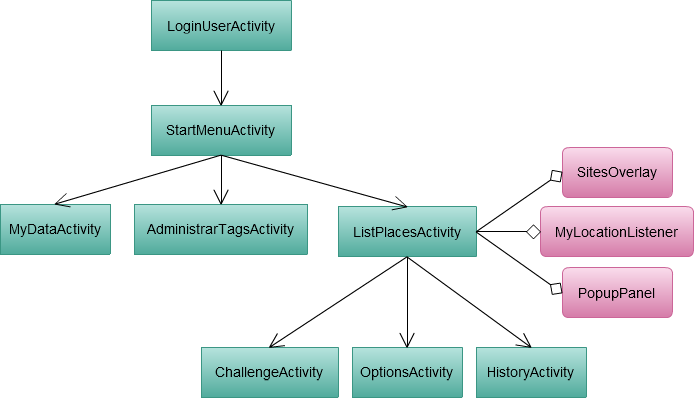
\includegraphics[width=400pt]{./imgs/TripdroidActivities.png}
\caption{Activities de la Aplicación}
\end{figure}

\newpage
Descripción de las Activities:\\

\paragraph{LoginUserActivity:} Contiene formulario para el registro y login de Usuario. Se valida enviando los datos de usuario y password al servidor para comprobar si el usuario existe.


\begin{figure}[h]
\hspace{3cm}
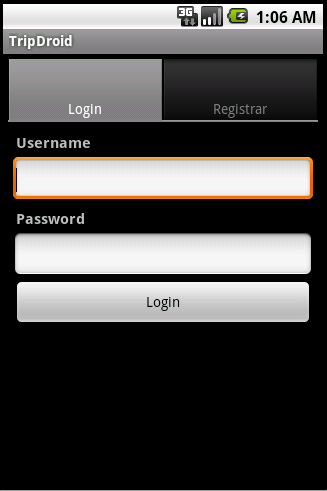
\includegraphics[width=180pt]{./imgs/TripdroidLogin.png}
\caption{Login y Registro}
\end{figure}

\newpage
\paragraph{StartMenuActivity:} Menu inicial que contiene enlaces a los Datos del Usuario, Ver el Mapa, o Administrar en caso de que el usuario sea un administrador.

\begin{figure}[h]
\hspace{3cm}
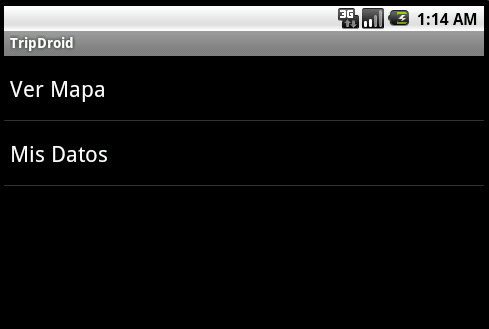
\includegraphics[width=180pt]{./imgs/TripdroidStartMenu.png}
\caption{Menú de Inicio}
\end{figure}

\paragraph{MyDataActivity:} Menú que resume los datos del usuario, su nombre, correo y experiencia.

\begin{figure}[h]
\hspace{3cm}
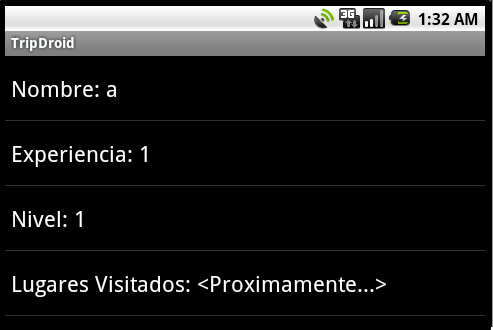
\includegraphics[width=180pt]{./imgs/TripdroidDatos.png}
\caption{Datos del Usuario}
\end{figure}

\newpage
\paragraph{AdministrarTagsActivity:} En caso de que el usuario sea un administrador, tiene acceso a esta actividad, la cual muestra una lista con los tags propuestos por los usuarios, además de los votos que han recibido como correctos o incorrectos para que el administrador pueda ingresarlos al sistema o no.

\begin{figure}[h]
\hspace{3cm}

\includegraphics[width=180pt]{./imgs/TripdroidAdmin.png}
\caption{Validación Tag}
\end{figure}

\paragraph{ListPlacesActivity:} Actividad que carga el Mapa y los lugares que estén cargados en la aplicación, con sus tags e información. El usuario puede visitar o agregar tags a los que se encuentren cercanos a su ubicación actual. Esta actividad funciona mediante las siguientes clases:\\

\begin{itemize}
 \item \textbf{SitesOverlay:} Clase que carga el mapa y los lugares.
 \item \textbf{MyLocationListener:} Thread que lee la ubicación actual del usuario mediante GPS
 \item \textbf{PopupPanel:} Ventana emergente con las coordenadas e información del lugar, y los botones que permiten realizar distintas acciones en el lugar al usuario.
\end{itemize}

\begin{figure}[h]
\hspace{3cm}
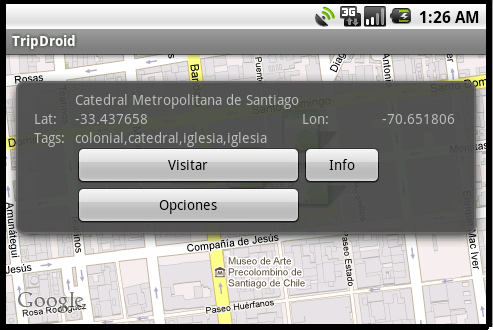
\includegraphics[width=180pt]{./imgs/TripdroidMapaMenu.png}
\caption{Mapa con Lugares}
\end{figure}

\newpage
\paragraph{ChallengeActivity:} Envía un desafío al usuario, en este caso, una pregunta acerca de si es correcta la relación entre un Lugar y un Tag.

\begin{figure}[h]
\hspace{3cm}
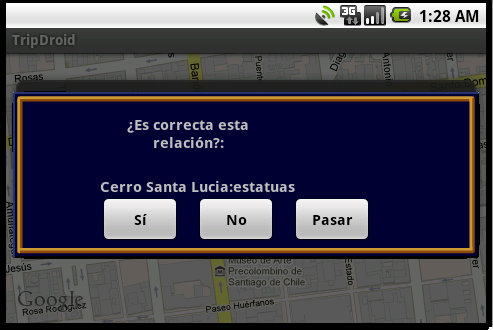
\includegraphics[width=180pt]{./imgs/TripdroidDesafio.png}
\caption{Desafío tipo Tag}
\end{figure}

\paragraph{OptionsActivity:} Aquí el usuario puede aportar datos acerca del Lugar, en el caso del prototipo, sólo puede proponer nuevos tags para el Lugar, que son posteriormente validados mediante desafíos para otros usuarios.

\begin{figure}[h]
\hspace{3cm}
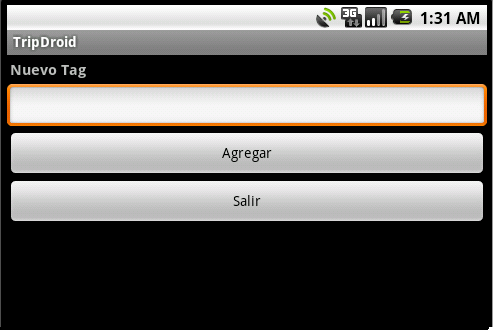
\includegraphics[width=180pt]{./imgs/TripdroidOpciones.png}
\caption{Agregar Tag}
\end{figure}

\paragraph{HistoryActivity:} Aún no desarrollada completamente. Actividad que muestra la historia o más información sobre el lugar.

\newpage
Además, existen otros 2 packages en la aplicación: Utils y Model\\

\paragraph{Model}

Contiene clases que son Objetos que corresponden a las distintas Tablas de la Base de Datos.(Place, User, DesafioTag).\\

\paragraph{Utils}

Contiene clases que se usan para desarrollar funcionalidades de las clases principales.\\

\begin{itemize}
 \item \textbf{InteractiveArrayAdapter:} Clase que adapta los arreglos de las ListView de Android para que tengan un CheckButton.
 \item \textbf{UserSession:} Maneja las sesiones de Usuario, contiene una instancia del objeto correspondiente al usuario actual en la aplicación.
 \item \textbf{WebServiceJSON:} Clase que permite obtener y enviar parámetros en formato de archivo JSON al servidor.
\end{itemize}

\subsubsection{Servidor}

El Servidor de la aplicación corresponde a un servidor gratuito de Google App Engine, donde se tienen los datos de los usuarios, lugares y desafíos y los distintos métodos para obtener dichos datos desde la aplicación cuando se requiera.\\

El modelo de datos es el siguiente:\\

\begin{figure}[h]
\hspace{1.5cm}
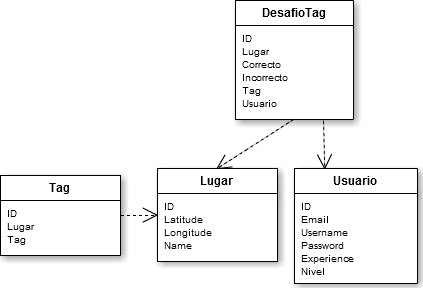
\includegraphics[width=220pt]{./imgs/ModeloDatos.png}
\caption{Agregar Tag}
\end{figure}

Y los métodos que tiene el Servidor son los siguientes: (todos los métodos reciben parámetros vía GET y retornan texto en formato JSON según lo que se requiera)\\

\begin{itemize}
\item \textbf{votaruntag():} Recibe como parámetro un tag y la respuesta del usuario al desafío asociado a ese tag (Sí o No) y le suma un punto al campo ‘correcto’ o ‘incorrecto’ de ese tag según corresponda.

\item \textbf{agregardesafiotag():} Al agregar un nuevo tag, éste método lo recibe como parámetro y crea el desafío asociado a la combinación lugar/tag/usuario, verificando que no exista previamente.

\item \textbf{obtenerdesafiotag():} Retorna un desafío al azar entre todos los desafíos que no hayan sido propuestos por el usuario que invoca el método. Esto es para generar la pregunta de la actividad del desafío.

\item \textbf{obtenertags():} Recibe como parámetro un lugar, y retorna los tags asociados al mismo.

\item \textbf{administrartags():} Retorna una lista de todos los desafíos de tags pendientes, junto con los votos que han recibido.

\item \textbf{agregarnuevotag():} Recibe como parámetro un tag que el administrador haya chequeado como correcto, luego, agrega este tag al lugar correspondiente y borra el desafío asociado a dicho tag.

\item \textbf{registrar():} Recibe como parámetros todos los datos del formulario de registro del usuario, y en caso de no existir un usuario con el mismo username, o email, lo registra en el sistema.

\item \textbf{login():} Recibe como parámetros el username y el password, verifica que la combinación sea correcta y le permite ingresar a la aplicación.

\end{itemize}

\subsection{Prueba con Usuarios}

Luego de elaborar el primer prototipo de la aplicación, éste fue mostrado a los usuarios utilizando un móvil Xperia Mini X10, mediante el cual probaron la aplicación, realizando las siguientes tareas:\\

\begin{itemize}
 \item Registrarse en la aplicación
 \item Visualizar el mapa
 \item Buscar un lugar cercano a su ubicación actual
 \item Visitarlo
 \item Responder un desafío
 \item Agregar un Tag
\end{itemize}


Posteriormente se le realizó una encuesta de usabilidad a los usuarios, donde evaluaron distintas característas en una escala de 1 a 5 (desde "Muy en Desacuerdo" hasta "Muy de Acuerdo"), y luego se permitía entregar feedback libre sobre la aplicación.\\

La encuesta fue realizada a 15 usuarios.\\

\subsubsection{Resultados Encuesta}

La escala fue normalizada de la siguiente forma:

\begin{itemize}
\item Muy en Desacuerdo : 1
\item En desacuerdo: 2
Neutro: 3
De acuerdo: 4
Muy de Acuerdo: 5\end{itemize}

Luego, el promedio de las respuestas de los encuestados en cada pregunta, fue el siguiente:\\

\begin{itemize}
\item La aplicación es fácil de usar \textbf{3,5}
\item Es fácil encontrar la información deseada \textbf{3,3}
\item Las distintas opciones funcionan correctamente \textbf{3,1}
\item Las velocidad de la aplicación es adecuada \textbf{3,4}
\item El uso del color es aceptable \textbf{3,4}
\item El diseño general de la aplicación es apropiado \textbf{3,2}
\item La organización de la información de la aplicación es apropiada \textbf{3,5}
\item El contenido de la aplicación es relevante \textbf{3,2}
\item La interfaz de la aplicación es placentera \textbf{3,2}
\item La aplicación tiene todas las funcionalidades esperadas \textbf{3}
\item La aplicación tiene todas las capacidades esperadas \textbf{3}
\item ¿Cómo califica globalmente la aplicación analizada? \textbf{3,2}

\item Promedio Total: \textbf{3,2}
\end{itemize}


\subsubsection{Feedback Usuarios}

Comentarios varios de los usuarios que probaron el prototipo y respondieron la encuesta, ordenados por los que se repitieron (o muy similares) más frecuentemente:\\

\begin{itemize}
\item Que los desafíos sean del lugar que visito (9 personas)
\item Permitir agregar nuevos lugares (8 personas)
\item Arreglar el focus del click en la ventana del lugar(8 personas)
\item Que no sea sólo landscape (8 personas)
\item Agregar búsqueda por tags (6 personas)
\item Que estén todos los lugares disponibles y la experiencia sirva para otra cosa (6 personas)
\item Botón para centrar el mapa (6 personas)
\item Tener familia de íconos propios de la app (5 personas)
\item Asociarlo a redes sociales(5 personas)
\item No se distingue bien en el desafío la parte de lugar::tag(4 personas)
\item Poner los Tags en Info en vez de la ventana emergente, o en ambos lugares. (3 personas)
\item Revisar lugares que visité (2 personas)
\item Revisar lugares que visitaron otros usuarios (2 personas)
\item Poner foto del lugare o ver galería de fotos de un lugar (2 personas)
\item Desbloquear ''easter eggs'' al ganar experiencia (2 personas)
\item Ejemplos del relleno en campos de texto
\item Menú Inicial que de Contexto
\item Pasar del registro directo a la app
\item Guardar username y pass
\item Texto de las ventanas emergentes más lento
\end{itemize}

\subsubsection{Análisis de Resultados}

Se puede apreciar que en general la evaluación de la aplicación es entre Neutro y De Acuerdo, más cercana al valor Neutro, lo cuál era esperable, ya que se hizo un prototipo bastante básico para empezar a probar. De hecho, sólo 3 usuarios de los encuestados evaluaron negativamente la aplicación globalmente.\\

En general, el principal problema con que se toparon los usuarios, fue que los desafíos no fueran relacionados directamente con el lugar que visitaban, sin embargo, la gran mayoría no tuvo inconveniente alguno en comprender intuitivamente lo que era el desafío en sí y que se utilizaba para validar, de hecho, varios de ellos mencionaron que era algo similar a lo que hacen varias aplicaciones en distintas redes sociales mientras probaban la aplicación.\\

Por último, se aprecia que la evaluación más baja es en el item ''La aplicación tiene todas las funcionalidades esperadas`` lo cuál es lógico puesto que se trata de un prototipo con el mínimo de funcionalidades. Esto es positivo, ya que los usuarios en general al ver la aplicación preguntaban por funcionalidades que les gustaría que tuviese o que creían que existían, las cuales se pueden ver en el resumen del feedback recibido, y permiten tener una guía para elaborar el segundo prototipo.\\

\newpage
\section{Propuesta Segundo Prototipo}

A raíz de los resultados obtenidos, para un segundo prototipo, el objetivo es tener las siguientes funcionalidades:\\

\begin{itemize}
\item Desafíos sólo relativos al lugar que se visita.
\item Permitir que el usuario agregue lugares.
\item Agregar alguna funcionalidad que se desbloquee al subir de nivel, por ejemplo, revisar lugares visitados.
\item Botón para centrar el mapa
\item Búsqueda de lugares por tag
\end{itemize}

\newpage
\section{Fases Posteriores}

Fuera del alcance del Trabajo Dirigido, se pretende seguir con el proyecto de la siguiente manera:\\

Realizar nuevamente un estudio de usabilidad basado en el segundo prototipo.\\

Elaborar un tercer prototipo, siendo este ya una primera versión definitiva de la aplicación.\\

Diseñar un Plan de Negocios, con ayuda de algún estudiante o profesional del área, pero que cubra más o menos la siguiente idea.\\

\textbf{Plan de Negocios:}\\

\begin{itemize}
 \item Terminar una versión definitiva de la aplicación basada en los resultados de este Trabajo Dirigido y posteriores encuestas a usuarios en las fases siguientes ya descritas.

  \item Dar a conocer la aplicación a empresas que apoyen ideas de innovación y les interese apoyar el proyecto (Cursor, CORFO, etc.).

 \item En esa misma línea, postular la aplicación al Concurso Kickstar de Innovación http://islae2.cl/.

 \item Conseguir usuarios para la aplicación, de modo de tener una base para decir que la aplicación es usada por la gente.

 \item Analizar que features utilizan los usuarios o las organizaciones contactadas para determinar si existen algunas por las cuáles les interesaría pagar (por ejemplo, por mayor acceso a datos sin necesidad de resolver desafíos, por publicidad dentro de la aplicación, o bien para entregar algún servicio a los clientes que usen la aplicación).

 \item Asimismo, utilizando como base el número de usuarios de la aplicación, buscar empresas que les interese tener auspicios en la aplicación.

\end{itemize}

\end{document}